\documentclass[10pt]{article}

\usepackage[a4paper, margin=1.4cm]{geometry}
\usepackage[utf8]{inputenc}
\usepackage[T1]{fontenc}
\usepackage{booktabs}
\usepackage{graphicx}
\usepackage{amsmath}
\usepackage{hyperref}
\usepackage{xcolor}
\usepackage{caption}
\usepackage{subcaption}
\usepackage{float}
\usepackage{array}
\usepackage{enumitem}
\usepackage{titlesec}

\captionsetup{font=footnotesize,labelfont=bf,skip=2pt}
\titlespacing*{\section}{0pt}{4pt}{2pt}
\titlespacing*{\subsection}{0pt}{3pt}{1pt}
\setlist{nosep,leftmargin=1.2em}
\setlength{\abovedisplayskip}{2pt}
\setlength{\belowdisplayskip}{2pt}
\pagestyle{empty}

\hypersetup{colorlinks=true,linkcolor=blue,citecolor=blue,urlcolor=blue}

\title{\large Beyond Pixels}
\date{\vspace{-1.5em}\small\today}

\begin{document}
\maketitle
\vspace{-1.5em}

\noindent\footnotesize
\textbf{Summary.} DenseNet-121 and ViT image-only models achieved mean test AUCs of nearly 0.73 for 21-label chest pathology classification on the Open-I
dataset. A multimodal fusion model combining a custom text encoder and a ViT via
bidirectional cross-attention reached a mean test AUC of 0.9886. 
Text/image tokens are projected to $d{=}512$; \textbf{t2i} (text queries $\times$
image kv) and \textbf{i2t} (image queries $\times$ text kv) cross-attentions run
in parallel, each followed by residual+LayerNorm+FFN. Pooled \texttt{[CLS]} text
and attention-pooled image vectors are concatenated and classified. Training:
two-phase (head-only warmup, epochs 1--3; full unfreeze, epochs 4--30), Asymmetric
Loss, early stop at epoch 22 (best val AUC 0.9881).



\vspace{2pt}
\begin{table}[H]
\centering\footnotesize
\caption{Model comparison -- mean test AUC.}
\begin{tabular}{lccc}
\toprule
Model & Backbone & Mean AUC & Notes \\
\midrule
DenseNet-121 & ImageNet pretrained & 0.72 & BCE (had overfit) \\
ViT v4 & \texttt{vit-chest-xray} & 0.7330 & Asymmetric Loss (no overfit) \\
\textbf{Fusion (Arch.\,1)} & Text(4.3M)+ViT(86M), 95.9M tot. & \textbf{0.9886} & Bidir. cross-attn, $d{=}512$, 8 heads \\
\bottomrule
\end{tabular}
\end{table}

\vspace{-4pt}
\section{Mediation Analysis}

Cross-modal mediation analysis suggests that this gain is largely driven by
\textbf{cross-modal information leakage}, whereby report information is injected
into the image representation through the Image$\rightarrow$Text cross-attention
pathway, rather than by genuinely improved visual understanding.
\textbf{Mediation method.} Each test sample is forward-passed with real and blank
report text, giving representation pairs
$(\text{text}_R,\text{image}_R)$ / $(\text{text}_B,\text{image}_B)$, recombined
through the shared head: \textit{real\_real} (full model), \textit{blankT+realI}
(text dropped, image already shaped by i2t on real text), \textit{realT+blankI}
(image dropped). ROC-AUC computed per condition over all 968 test samples, 21 labels.

\begin{table}[H]
\centering\footnotesize
\caption{Mediation analysis -- mean AUC across 21 pathologies ($n=968$).}
\begin{tabular}{lccc}
\toprule
real\_real (full model) & blankT+realI & realT+blankI & $\Delta$(real$-$blankT+realI) \\
\midrule
0.9833 & 0.9824 & 0.7648 & $+0.0010$ \\
\bottomrule
\end{tabular}
\end{table}

\vspace{-4pt}
\textbf{Interpretation.} Dropping text while keeping an i2t-shaped image
representation costs $\approx$0 AUC (even slightly negative for 7/21 classes) --
the image with the i2t part carries the most important signal used by the model.


\vspace{2pt}
\begin{figure}[H]
\centering
\begin{subfigure}{0.30\textwidth}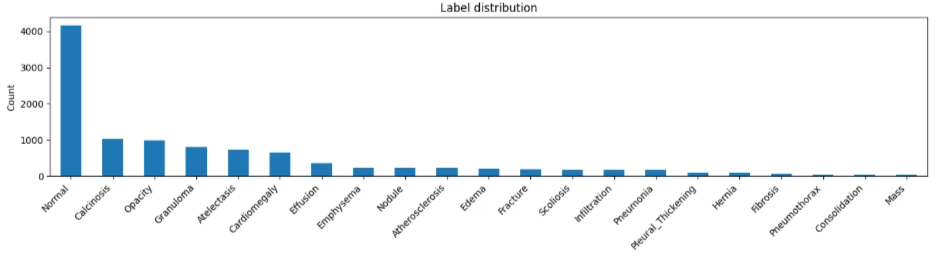
\includegraphics[width=\linewidth]{figures/dataset.png}\caption{Label distribution}\end{subfigure}
\hfill
\begin{subfigure}{0.30\textwidth}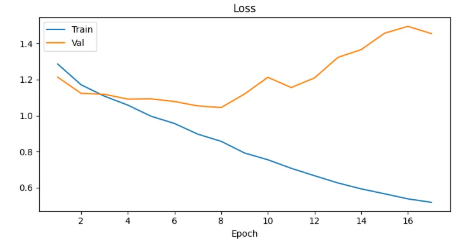
\includegraphics[width=\linewidth]{figures/densenet_loss_func.png}\caption{DenseNet-121 loss}\end{subfigure}
\hfill
\begin{subfigure}{0.30\textwidth}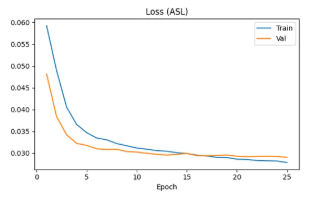
\includegraphics[width=\linewidth]{figures/ViT_final_loss_func.png}\caption{ViT training loss (ASL)}\end{subfigure}
\\[3pt]
\begin{subfigure}{0.60\textwidth}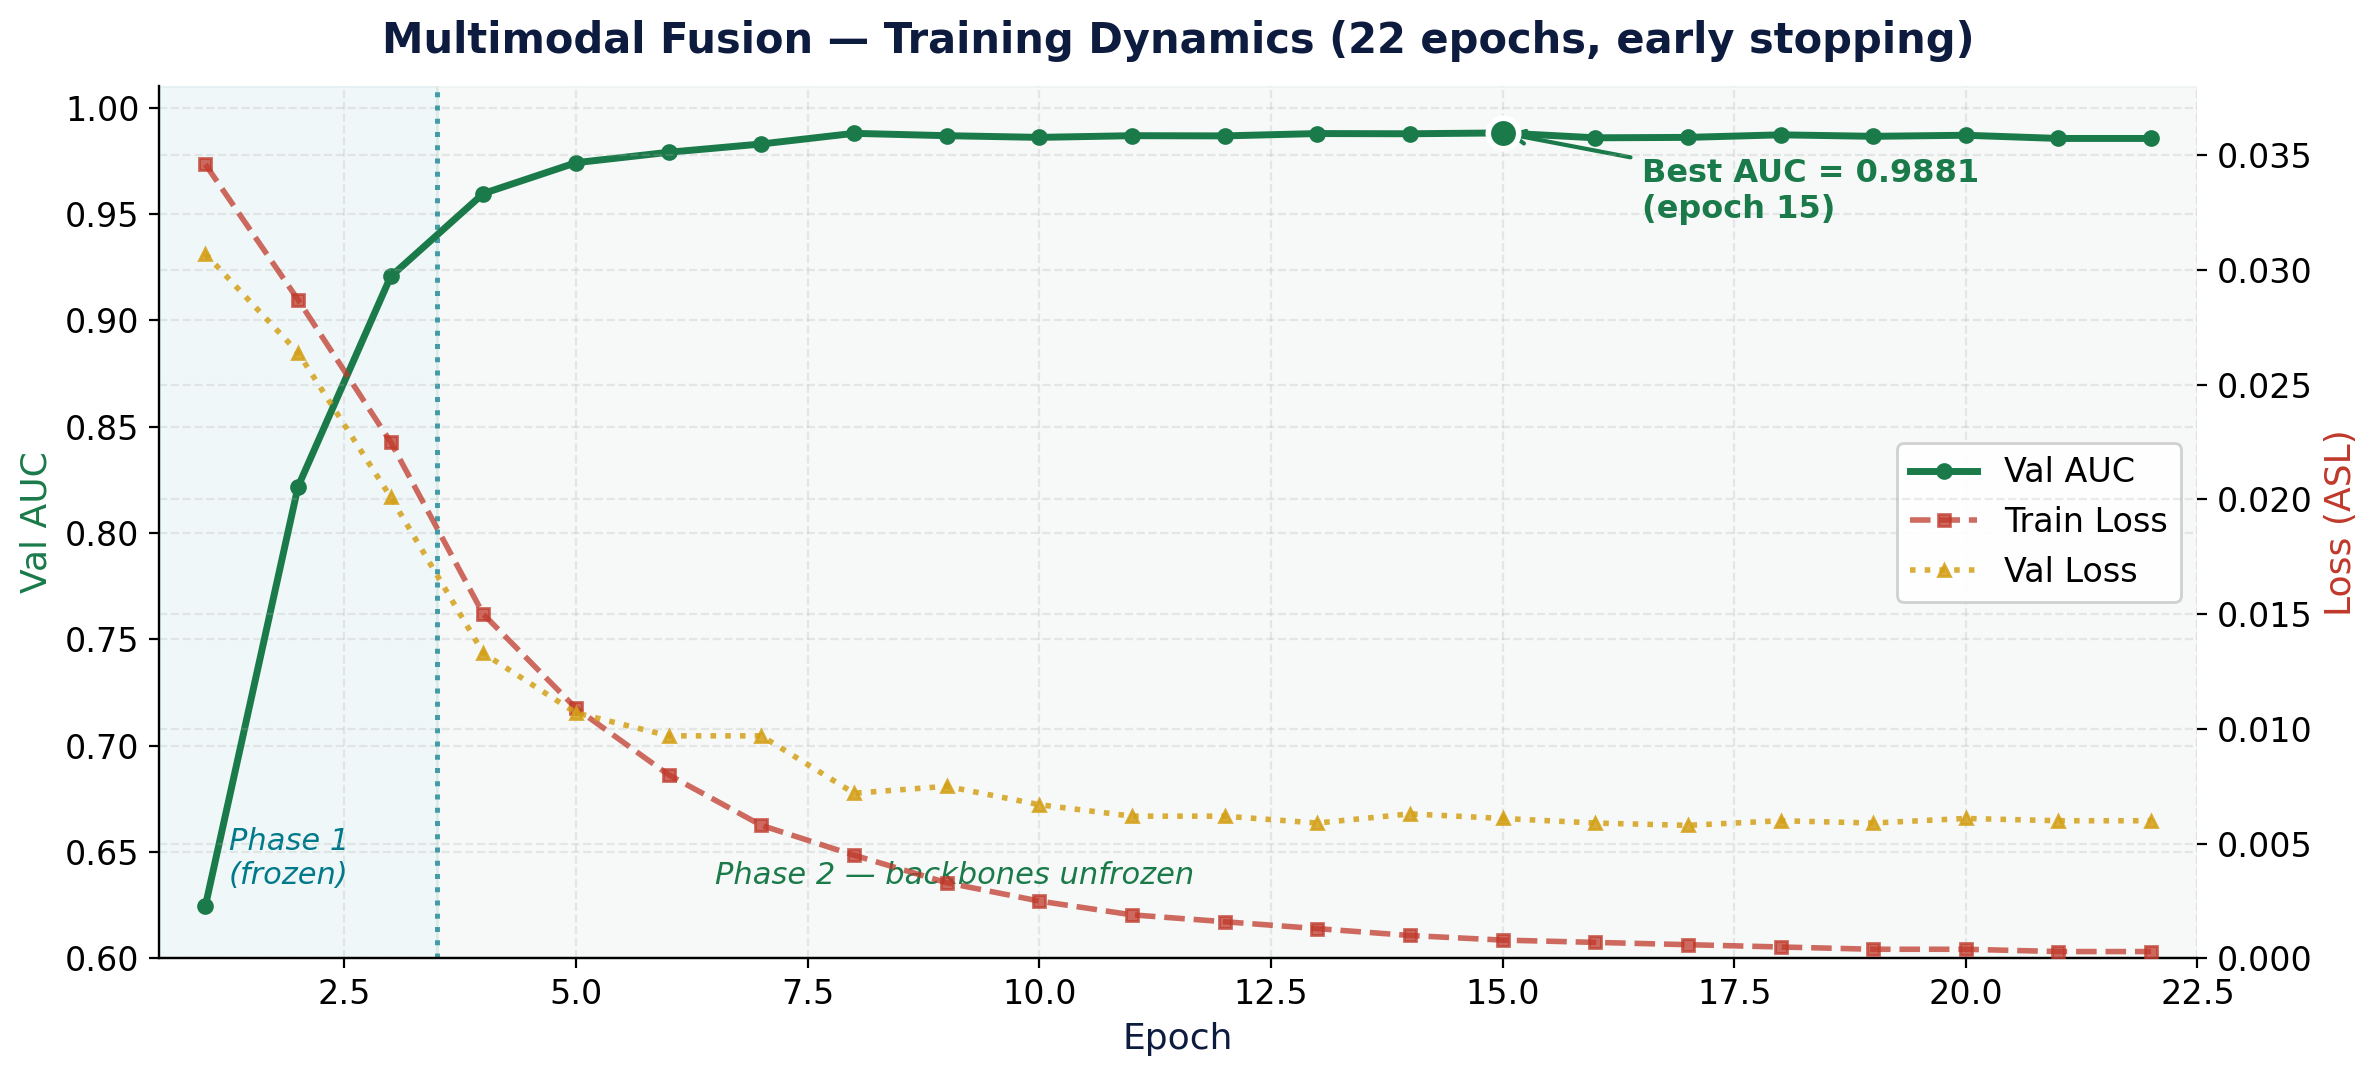
\includegraphics[width=\linewidth]{figures/fig3_training_curve_multi_modal.png}\caption{Fusion training/val AUC}\end{subfigure}
\hfill
\begin{subfigure}{0.3\textwidth}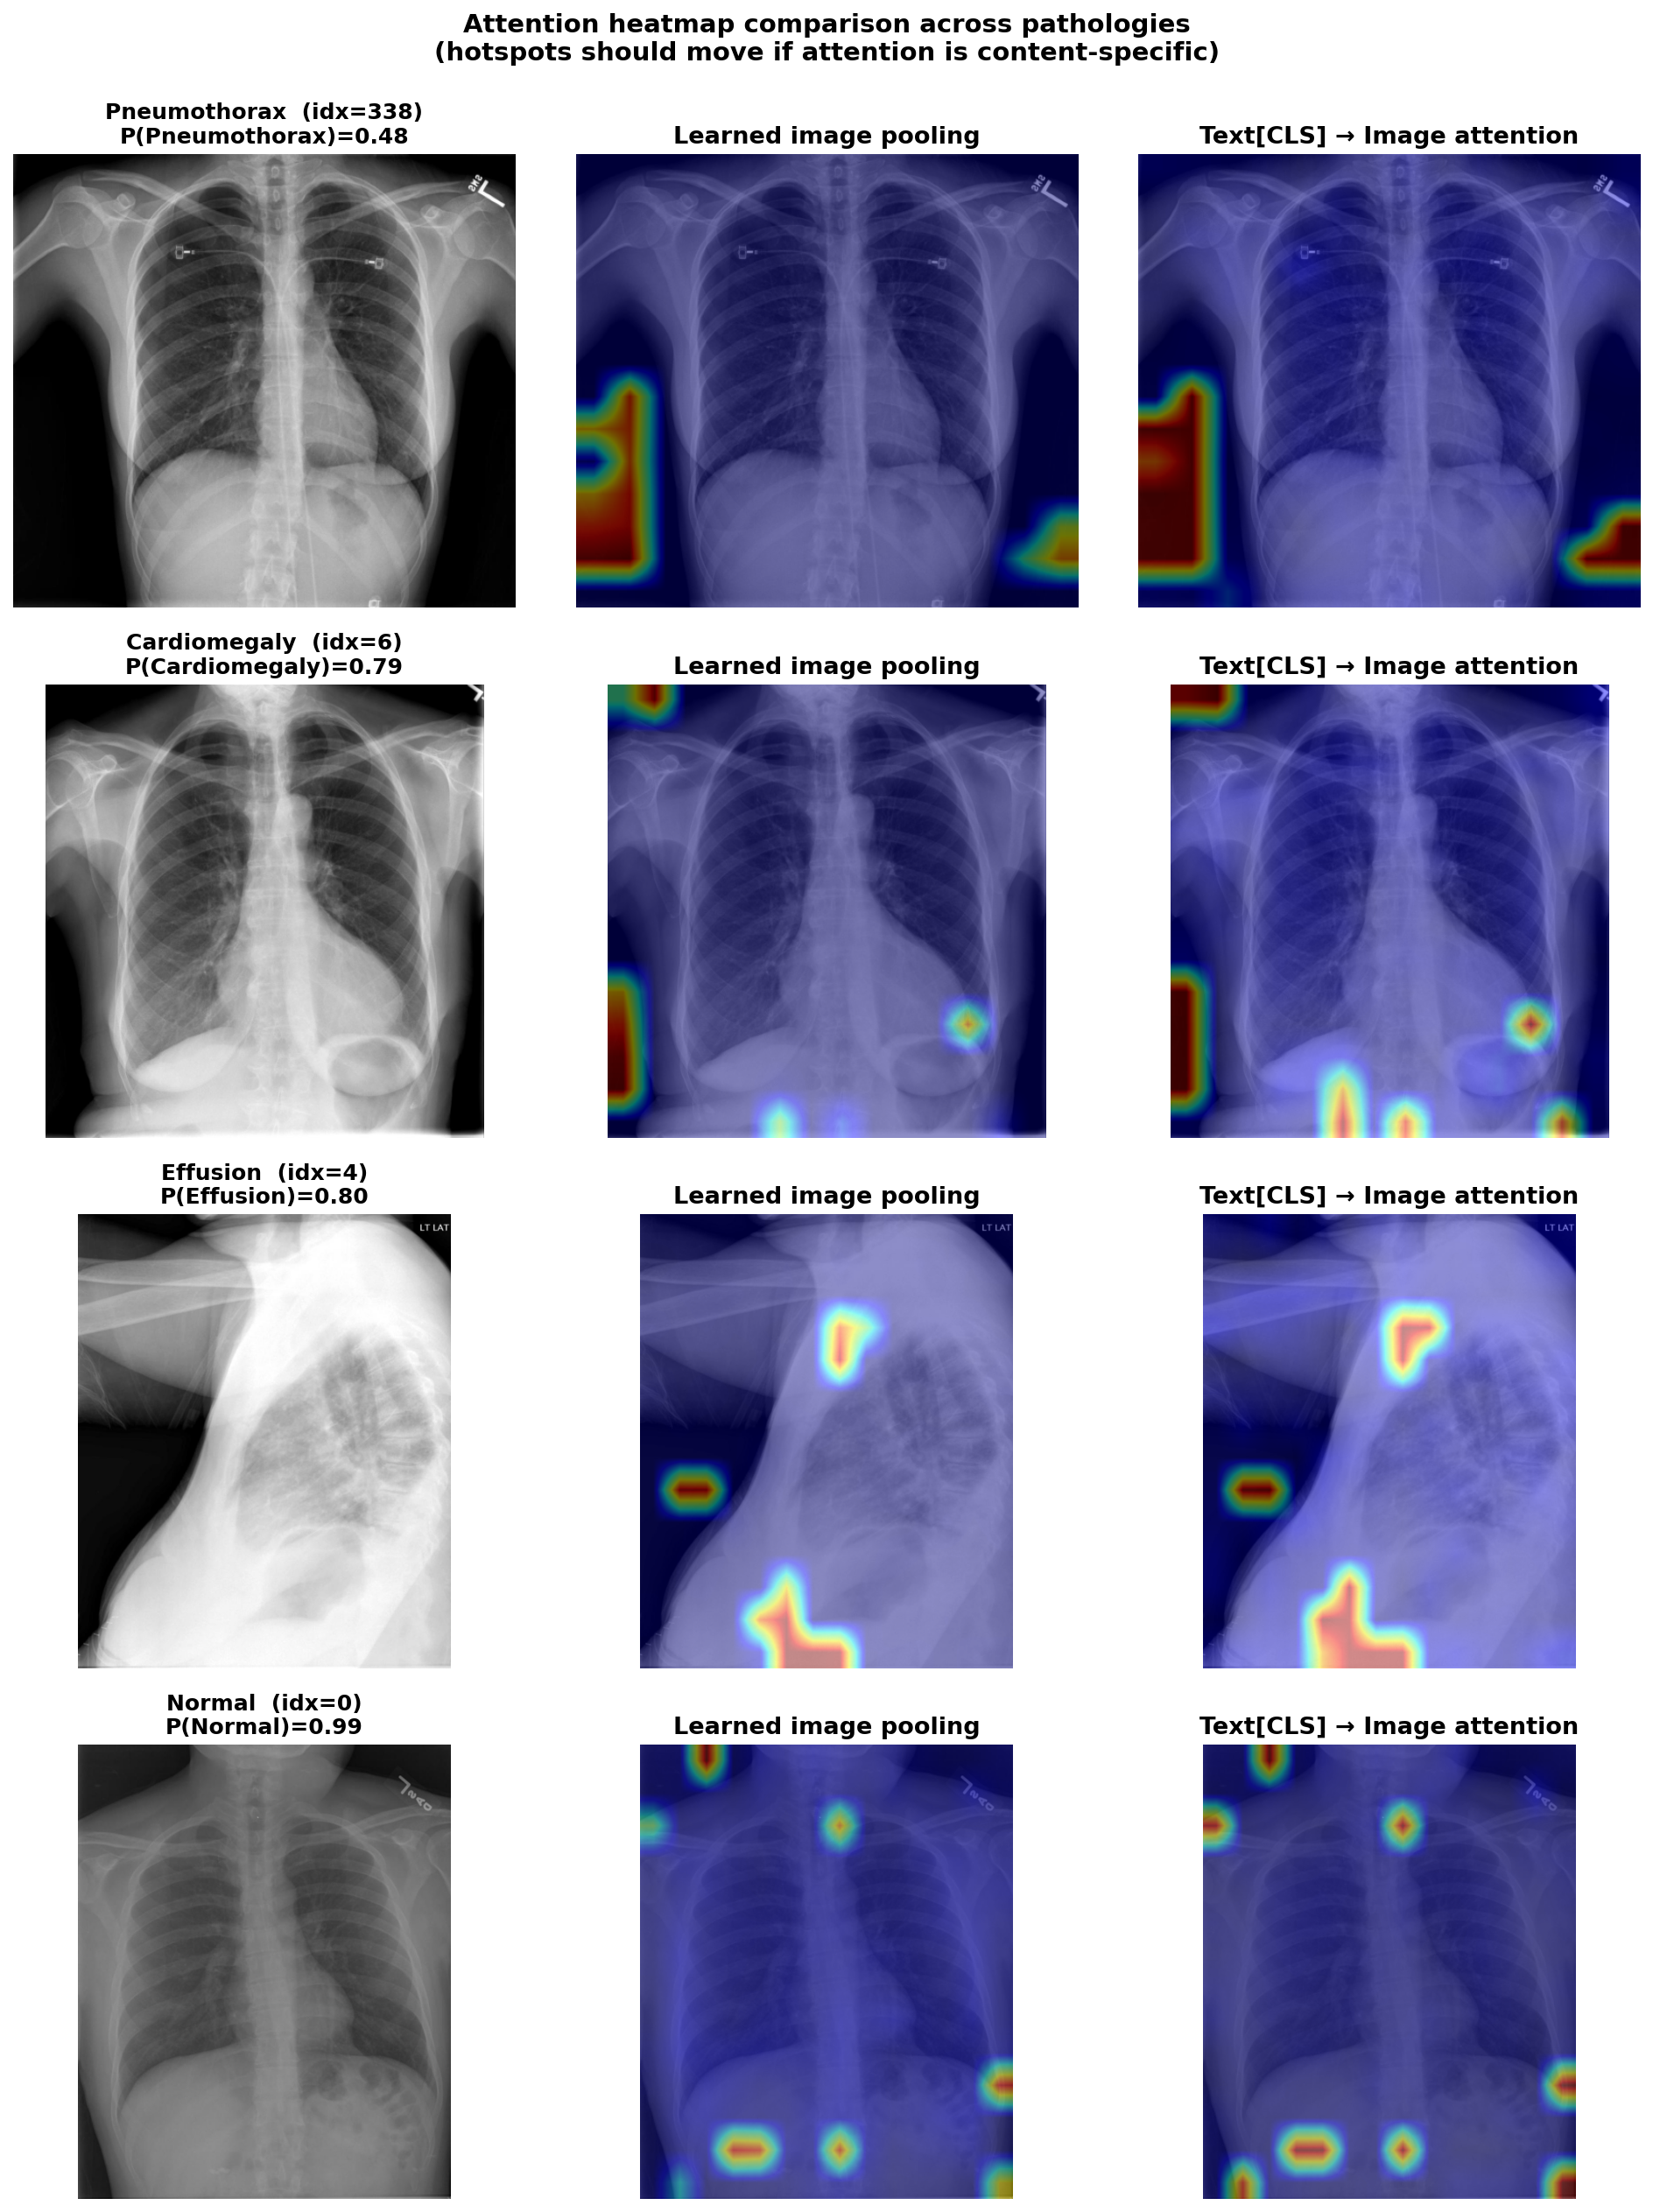
\includegraphics[width=\linewidth]{figures/attention_comparaison.png}\caption{Attention heatmaps: pooling (mid) vs.\ i2t cross-attn (right)}\end{subfigure}
\caption{Key figures across image-only training (a--c) and multimodal fusion (d--e).}
\end{figure}

\end{document}
